\ifdefined\ishandout
\documentclass[handout]{beamer}
\else
\documentclass{beamer}
\fi

\usepackage[frenchb]{babel}
\usepackage[T1]{fontenc}
\usepackage[latin1]{inputenc}
\usepackage{hyperref}
\usepackage{multirow}
\usepackage{listings}
\usepackage{fancyvrb}
\usepackage{tikz}
\usepackage{framed}
\usepackage{algorithm}
\usepackage{algorithmic}
\usepackage{xcolor}
\usepackage{color, colortbl}
\usepackage{handoutWithNotes}
\usepackage{amsmath}
\usetikzlibrary{shapes.geometric}
\usetikzlibrary{positioning}
\usetikzlibrary{shapes.arrows, chains}
\usetikzlibrary{arrows,calc}
\usetikzlibrary{shapes.multipart}
\usepackage{array}
\usetheme{Boadilla}
\definecolor{BlueGreen}{cmyk}{0.85,0,0.33,0}
\definecolor{Gray}{rgb}{0.8,0.8,0.8}

\ifdefined\ishandout
\pgfpagesuselayout{3 on 1 with notes}[a4paper,border shrink=5mm]
\usecolortheme{dove}
\else
\usecolortheme{dolphin}
\fi


\lstnewenvironment{codeC}
{ \lstset{language=C,
    otherkeywords={printf,scanf}}
}
{}

\ifdefined\ishandout
\definecolor{mygreen}{rgb}{0,0,0}
\definecolor{mymauve}{rgb}{0,0,0}
\definecolor{myblue}{rgb}{0,0,0}
\else
\definecolor{mygreen}{rgb}{0,0.6,0}
\definecolor{mymauve}{rgb}{0.58,0,0.82}
\definecolor{myblue}{rgb}{0,0,1}

\fi

\definecolor{mygray}{rgb}{0.5,0.5,0.5}


\lstset{language=C,
% breakatwhitespace=false,         % sets if automatic breaks should only happen at whitespace
%  breaklines=true,                 % sets automatic line breaking
%  captionpos=b,                
commentstyle=\itshape\color{mymauve},
keywordstyle=\bfseries\color{myblue},
%numbers=left,                    % where to put the line-numbers; possible values are (none, left, right)
%  numbersep=8pt,                   % how far the line-numbers are from the code
%  numberstyle=\tiny\color{mygray}, % the style that is used for the line-numbers
  rulecolor=\color{black},         % if not set, the frame-color may be changed on line-breaks within not-black text (e.g. comments (green here))
%  showspaces=false,                % show spaces everywhere adding particular underscores; it overrides 'showstringspaces'
  showstringspaces=false,          % underline spaces within strings only
%  showtabs=false,                  % show tabs within strings adding particular underscores
%  stepnumber=2,                    % the step between two line-numbers. If it's 1, each line will be numbered
  stringstyle=\color{mygreen},     % string literal style
%  tabsize=2 
}
\ifdefined\ishandout
\newcommand{\red}{\textbf}
\else
\newcommand{\red}{\textcolor{red}}
\fi
%\newcommand \emph
%Default size : 12.8 cm * 9.6 cm

\newcommand{\tmark}[1]{\tikz[remember picture, baseline=-.5ex]{\coordinate(#1);}}

\ifdefined\ishandout
\newenvironment<>{codeblock}[1]{%begin
  \setbeamercolor{block title}{fg=black,bg=lightgray!80}%
  \begin{block}{#1}}
  % \begin{codeC}}
  %  {\end{codeC}
{  
\end{block}}

\newenvironment<>{termblock}[1]{
    \setbeamercolor{block title}{fg=black,bg=lightgray!90}%
    \begin{block}{#1}
}
%     \begin{Verbatim}}
{%\end{Verbatim}
\end{block}
}

\definecolor{bluegreen}{RGB}{0,0,0}
%\definecolor{bluegreen}{rgb}{0,0.6,0.8}
\else

\newenvironment<>{codeblock}[1]{%begin
  \setbeamercolor{block title}{fg=darkgray,bg=yellow}%
  \begin{block}{#1}}
  % \begin{codeC}}
  %  {\end{codeC}
{  
\end{block}}

\newenvironment<>{termblock}[1]{
    \setbeamercolor{block title}{fg=white,bg=lightgray}%
    \begin{block}{#1}}
%     \begin{Verbatim}}
{%\end{Verbatim}
\end{block}
}

\definecolor{bluegreen}{RGB}{0,149,182}
%\definecolor{bluegreen}{rgb}{0,0.6,0.8}
\fi

%\newcommand{\output}[1]{
\setbeamertemplate{navigation symbols}{}
\newcommand{\bvrb}{\Verb[commandchars=���,formatcom=\color{bluegreen}]}
\newcommand{\footvrb}{\footnotesize\Verb}
\newcommand{\vrbalert}[2][]{\visible<#1>{#2}}
%%% Commande pour les listes/arbres
\newcommand{\mvide}{\nodepart{one} \nodepart{two}}
\newcommand{\tvide}{\nodepart{one} \nodepart{two} \nodepart{three}}

%%Fin des commandes pour les listes/arbres.


\newcommand<>{\case}[2]{%
\filldraw (#1,#2) rectangle (1+#1,1+#2);}
%%% Param�tres du cours (� r�gler)
%Num�ro du cours
\newcommand{\nb}{9}
\title[cours n�8]{Sujets avanc�s-2}
\author[]{julien.brajard@upmc.fr}
\institute[Polytech'UPMC]{Polytech'UPMC}
\date{20 Novembre 2017}
\begin{document}

\begin{frame}
\titlepage
\centering{
\url{https://moodle-sciences.upmc.fr} (cours Informatique G�n�rale MAIN-ROB)}
\end{frame}

\begin{frame}
\frametitle{Plan du cours}
\tableofcontents[hideallsubsections]
\end{frame}
% !TEX encoding = IsoLatin9
\section{L'algorithme A*}\label{section:2}
\begin{frame}
  \begin{columns}
    \column{4.8cm}
    \tableofcontents[currentsection,hideothersubsections]
    \column{7cm}
    \centering{
      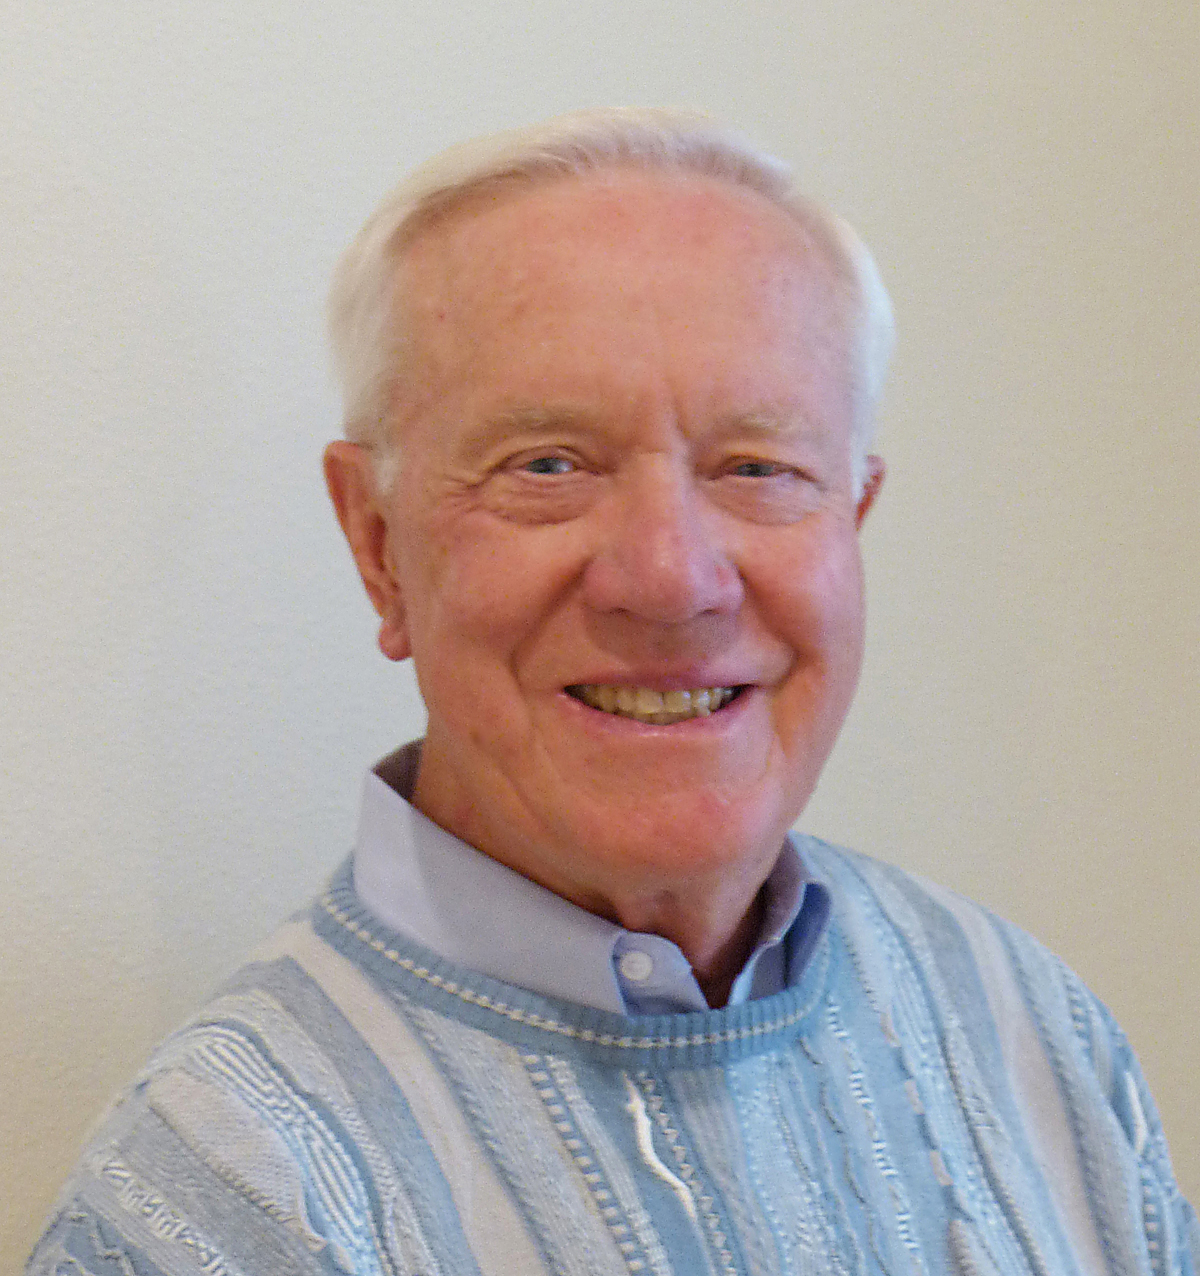
\includegraphics[width=4cm]{fig/Nils.jpg}
      
      \textit{``The point of all this is to be able to spend more time at the beach!''}\\
      \small{
        \hfill Nils Nilsson (1933-), inventeur de l'algorithme A*
              }
    }
  \end{columns}
  
\end{frame}

\begin{frame}
\frametitle{Probl�me pos�}
\begin{block}{Probl�me du Labyrinthe}
Sur une grille, on cherche � trouver le chemin le plus court du point D au point A
sachant qu'il y a des obstacles.
\end{block}
\begin{columns}
\column{0.55\textwidth}
Ce qu'on connait :
\begin{itemize}
\item Les noeuds accessibles (en blanc) et les noeuds inaccessibles (en noir)
\item Les voisins de chaque noeud (dans notre ex : noeuds du haut, du bas, de gauche, de droite).
\item Le co�t pour aller d'un noeud � son voisin (ici : 1 pour tous les noeuds).
\end{itemize}

\column{0.45\textwidth}
\begin{tikzpicture}[x=1cm,scale=0.75]
  \foreach \y in {0,...,7}{
    \foreach \x in {0,...,6}{
        \draw [black,thick, black] (\x,\y) rectangle (1+\x,1+\y);}}

\begin{scope}[fill=black, draw=black, thick]
  \case{4}{2};
  \case{4}{3};
  \case{4}{4};
  \case{3}{2};
  \case{3}{1};
  \case{3}{4};
  \case{2}{4};
  \case{0}{1};
  \case{1}{1};
  \case{2}{1};
\end{scope}


\node [anchor = center] at (0.5,3.5) {\Large{D}};
\node [anchor = center] at (5.5,3.5) {\Large{A}};

\end{tikzpicture}

\end{columns}
\end{frame}

\begin{frame}
\frametitle{Un algorithme possible : A*}
\begin{block}{}
L'algorithme A* permet de trouver rapidement le chemin le plus court.
Il s'agit de l'extension d'un autre algorithme : l'algorithme de Dijkstra.
\end{block}

Il est tr�s utilis� en intelligence artificielle (d�placement de robot, jeux vid�os).

\begin{alertblock}{}
Il est n�cessaire d'introduire des donn�es suppl�mentaires au probl�me initial
\end{alertblock}

\end{frame}

\begin{frame}[fragile]
\frametitle{Quelles informations suppl�mentaires ajouter ?}
\begin{block}{La structure case}
Plusieurs champs doivent �tre indiqu�es dans une case :
\begin{itemize}
\item Les coordonn�es : $x,y$
\item Le co�t pour se rendre du d�part � cette case : cost
\item Une estimation du co�t total (=cost + estimation de la distance restante) : heuristique
\item Les coordonn�es du noeud d'o� l'on vient.
\end{itemize}
\end{block}
\begin{codeblock}{}
\vspace{-.3cm}
\lstset{escapeinside={��}}
%\lstset{basicstyle=\scriptsize}
\begin{codeC}
struct case {
  int x,y; 
  float cost ; 
  float heuristique ;
  int xp,yp ; //noeud pr�c�dent
  } ;
  
\end{codeC}
\vspace{-.3cm}
\end{codeblock}
\end{frame}

\begin{frame}
\frametitle{Calcul de l'heuristique}
\begin{columns}
\column{.48\textwidth}
\begin{block}{Estimation de la distance restante}
G�n�ralement, elle est estim�e comme le co�t du chemin le plus court sans obstacle
("� vol d'oiseau").
\end{block}
L�gende :
\begin{itemize}
\item D d�signe le point de d�part
\item A d�signe le point d'arriv�e
\item $\leftarrow$ d�signe la case pr�c�dente
\item le couple de nombres d�finit les valeurs (cout,heuristique).
\end{itemize}
%\begin{columns}
%\column{0.5}

\column{0.52\textwidth}
\begin{tikzpicture}[x=1cm,scale=0.9]
  \foreach \y in {0,...,7}{
    \foreach \x in {0,...,6}{
        \draw [black,thick, black] (\x,\y) rectangle (1+\x,1+\y);}}

\begin{scope}[fill=black, draw=black, thick]
  \case{4}{2};
  \case{4}{3};
  \case{4}{4};
  \case{3}{2};
  \case{3}{1};
  \case{3}{4};
  \case{2}{4};
  \case{0}{1};
  \case{1}{1};
  \case{2}{1};
\end{scope}

%Arraow
\begin{scope}[<-,black, very thick]
\draw  (0.8,3.5) -- (1.2,3.5);
\draw  (1.8,3.5) -- (2.2,3.5);
\draw [->, red,very thick] (2.5,3.5) -- node[above,xshift=1]{\Large{\textbf{3}}} (5.5,3.5);
\end{scope}

\node [anchor = center] at (1.5,3.5) {\footnotesize{(1,5)}};
\node [anchor = center] at (2.5,3.5) {\footnotesize{(2,5)}};
\node [anchor = center] at (0.5,3.5) {\Large{D}};
\node [anchor = center] at (5.5,3.5) {\Large{A}};

\end{tikzpicture}
\end{columns}
\end{frame}


\begin{frame}
\frametitle{Les diff�rentes listes}
Dans l'algorithme A*, on s�pare les cases en diff�rentes cat�gories :
\begin{itemize}
\item Les cases non explor�es : ces cases sont les cases pour lesquels on n'a pas encore calcul�
la valeur (cout, heuristique, etc.)
\item Les cases � explorer : ces cases sont stock�es dans une liste, l'\textcolor{green}{openList}. On a calcul� leur valeurs mais on ne les a pas encore explor�es.
\item Les cases d�j� explor�es : ces cases sont stock�es dans une liste, la \textcolor{red}{closedList}. On a calcul� leurs valeurs et aussi les valeurs de leurs voisines.
\end{itemize}

\end{frame}


\begin{frame}
\frametitle{Algorithme A*}
\begin{columns}
\column{.48\textwidth}
\begin{itemize}
\item \alert<2>{\textcolor{red}{closedList} = \{\}, \textcolor{green}{openList} = D}
\item Tant que openList non vide
\begin{itemize}
\item \alert <3-18>{c : prendre le plus petit �l�ment de openList et l'ajout� � la closedList.}
\item \alert <18> {si c est l'objectif A : reconstituer le chemin et le renvoyer}
\item \alert <3-17>{sinon : ajouter les voisins de c non explor�s dans l'OpenList}
\end{itemize}
\item Si l'openList est vide: pas de chemin possible.
\end{itemize}

\column{0.52\textwidth}

\begin{tikzpicture}[x=1cm,scale=0.9]
  \foreach \y in {0,...,7}{
    \foreach \x in {0,...,6}{
        %fill (\x,\y) rectangle (1+\x,1+\y) rectangle (2+\x,2+\y);}}
        \draw [black,thick, black] (\x,\y) rectangle (1+\x,1+\y);}}

\begin{scope}[fill=black, draw=black, thick]
  \case{4}{2};
  \case{4}{3};
  \case{4}{4};
  \case{3}{2};
  \case{3}{1};
  \case{3}{4};
  \case{2}{4};
  \case{0}{1};
  \case{1}{1};
  \case{2}{1};
\end{scope}

%Open list
\begin{scope}[fill=green, draw=black, thick]
\filldraw <2> (0,3) rectangle(1,4);
\filldraw <3-> (1,3) rectangle(2,4);
\filldraw <3-> (0,4) rectangle(1,5);
\filldraw <3-> (0,2) rectangle(1,3);
\filldraw <4-> (1,4) rectangle(2,5);
\filldraw <4-> (1,2) rectangle(2,3);
\filldraw <4-> (2,3) rectangle(3,4);
\filldraw <5-> (2,2) rectangle(3,3);
\filldraw <5-> (3,3) rectangle(4,4);
\filldraw <7-> (1,5) rectangle(2,6);
\filldraw <8-> (0,5) rectangle(1,6);
\filldraw <12-> (2,5) rectangle(3,6);
\filldraw <12-> (1,6) rectangle(2,7);
\filldraw <13-> (2,6) rectangle(3,7);
\filldraw <13-> (3,5) rectangle(4,6);
\filldraw <14-> (4,5) rectangle(5,6);
\filldraw <14-> (3,6) rectangle(4,7);
\filldraw <15-> (5,5) rectangle(6,6);
\filldraw <15-> (4,6) rectangle(5,7);
\filldraw <16-> (6,5) rectangle(7,6);
\filldraw <16-> (5,6) rectangle(6,7);
\filldraw <16-> (5,4) rectangle(6,5);
\filldraw <17-> (5,3) rectangle(6,4);
\filldraw <17-> (6,4) rectangle(7,5);

\end{scope}

%Closed list
\begin{scope}[fill=red, draw=black, thick]
\filldraw <3-> (0,3) rectangle(1,4);
\filldraw <4-> (1,3) rectangle(2,4);
\filldraw <5-> (2,3) rectangle(3,4);
\filldraw <6-> (3,3) rectangle(4,4);
\filldraw <7-> (1,4) rectangle(2,5);
\filldraw <8-> (0,4) rectangle(1,5);
\filldraw <9-> (0,2) rectangle (1,3);
\filldraw <10-> (1,2) rectangle (2,3);
\filldraw <11-> (2,2) rectangle (3,3);
\filldraw <12-> (1,5) rectangle(2,6);
\filldraw <13-> (2,5) rectangle(3,6);
\filldraw <14-> (3,5) rectangle(4,6);
\filldraw <15-> (4,5) rectangle(5,6);
\filldraw <16-> (5,5) rectangle(6,6);
\filldraw <17-> (5,4) rectangle(6,5);
\filldraw <18-> (5,3) rectangle(6,4);

\end{scope}

%Arraow
\begin{scope}[<-,black, very thick]
\draw <3-> (0.8,3.5) -- (1.2,3.5);
\draw <3-> (0.5,3.8) -- (0.5,4.2);
\draw <3-> (0.5,3.2) -- (0.5,2.8);

\draw <4-> (0.8,3.5) -- (1.2,3.5);
\draw <5-> (1.8,3.5) -- (2.2,3.5);
\draw <6-> (2.8,3.5) -- (3.2,3.5);
\draw <7-> (1.5,3.8) -- (1.5,4.2);
\draw <10-> (1.5,3.2) -- (1.5,2.8);
\draw <11-> (2.5,3.2) -- (2.5,2.8);
\draw <12-> (1.5,4.8) -- (1.5,5.2);
\draw <13-> (1.8,5.5) -- (2.2,5.5);
\draw <14-> (2.8,5.5) -- (3.2,5.5);
\draw <15-> (3.8,5.5) -- (4.2,5.5);
\draw <16-> (4.8,5.5) -- (5.2,5.5);
\draw <17-> (5.5,5.2) -- (5.5,4.8);
\draw <18-> (5.5,4.2) -- (5.5,3.8);

\end{scope}

\node <3-> [anchor = center] at (1.5,3.5) {\footnotesize{(1,5)}};
\node <3-> [anchor = center] at (0.5,2.5) {\footnotesize{(1,7)}};
\node <3-> [anchor = center] at (0.5,4.5) {\footnotesize{(1,7)}};
\node <4-> [anchor = center] at (2.5,3.5) {\footnotesize{(2,5)}};
\node <4-> [anchor = center] at (1.5,2.5) {\footnotesize{(2,7)}};
\node <4-> [anchor = center] at (1.5,4.5) {\footnotesize{(2,7)}};
\node <5-> [anchor = center] at (2.5,2.5) {\footnotesize{(3,7)}};
\node <5-> [anchor = center] at (3.5,3.5) {\footnotesize{(3,5)}};
\node <7-> [anchor = center] at (1.5,5.5) {\footnotesize{(3,9)}};
\node <8-> [anchor = center] at (0.5,5.5) {\footnotesize{(2,9)}};
\node <12-> [anchor = center] at (1.5,6.5) {\footnotesize{(4,11)}};
\node <12-> [anchor = center] at (2.5,5.5) {\footnotesize{(4,9)}};
\node <13-> [anchor = center] at (2.5,6.5) {\footnotesize{(5,11)}};
\node <13-> [anchor = center] at (3.5,5.5) {\footnotesize{(5,9)}};
\node <14-> [anchor = center] at (3.5,6.5) {\footnotesize{(6,11)}};
\node <14-> [anchor = center] at (4.5,5.5) {\footnotesize{(6,9)}};
\node <15-> [anchor = center] at (4.5,6.5) {\footnotesize{(7,11)}};
\node <15-> [anchor = center] at (5.5,5.5) {\footnotesize{(7,9)}};
\node <16-> [anchor = center] at (5.5,6.5) {\footnotesize{(8,11)}};
\node <16-> [anchor = center] at (6.5,5.5) {\footnotesize{(8,11)}};

\node <16-> [anchor = center] at (5.5,4.5) {\footnotesize{(8,9)}};
\node <17-> [anchor = center] at (6.5,4.5) {\footnotesize{(9,11)}};

\draw <18> [gray,ultra thick] (0.5,3.5) -- (1.5,3.5) -- (1.5,5.5) -- (5.5,5.5) -- (5.5,3.5);

\node [anchor = center] at (0.5,3.5) {\Large{D}};
\node [anchor = center] at (5.5,3.5) {\Large{A}};

\end{tikzpicture}

\end{columns}
\end{frame}

\begin{frame}[fragile]
\frametitle{Comment ajouter un voisin dans l'openList ?}
\begin{codeblock}{}
\vspace{-.3cm}
\lstset{escapeinside={��}}
\lstset{basicstyle=\small}
\begin{codeC}
struct case nouvelle_case (struct case c,int x, int y) {

  struct case v; //case voisine de c
  v.x = x;
  v.y = y;
  v.cost = c.cost+1;
  v.heuristique = v.cost + estimation_distance(x,y);
  v.xp = c.x;
  v.yp = c.y;
  return v;
}
\end{codeC}
\vspace{-.3cm}
\end{codeblock}
\end{frame}

% !TEX encoding = IsoLatin9

%%%%%%%%%%%%%%%%%%%%% SECTION 1
\section{L'algorithme minimax}

\begin{frame}
\frametitle{L'algorithme minimax}
\begin{itemize}
\setlength\itemsep{1em}
\item Algorithme issu de la th�orie des jeux
\item Il s'applique aux jeux � 2 joueurs, �  somme nulle
(1 gagnant/1perdant ou match nul) et � information compl�te.
\end{itemize}

\begin{block}{Principe}
Passer en revu un nombre limit� de coups
et les �valuer en fonction du b�n�fice pour le joueur
et sont adversaire
\end{block}

\end{frame}

\begin{frame}
\frametitle{Evaluation d'un position}
\begin{columns}
\column{0.7\textwidth}
\begin{figure}
\centering
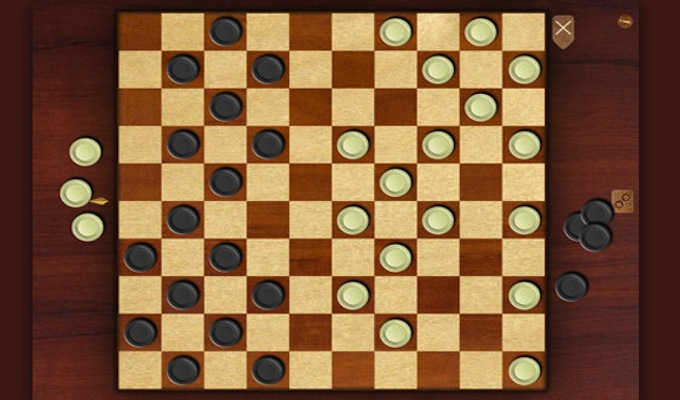
\includegraphics[width=8cm]{./fig/dames.jpg}
\end{figure}
\column{0.25\textwidth}
Joueur : Blancs\\
Adversaires : Noirs \\
\end{columns}
\vspace{1em}
Evaluation = Nbre de pions blancs - Nbre de pions noirs (ici = 1)
\end{frame}

\begin{frame}
\frametitle<1-8|handout:1-2>{Arbre minimax}
\frametitle<9-|handout:3>{Variante Negamax}
\begin{figure}
\begin{tikzpicture} [
  remember picture,
  auto,
  noeud/.style = {circle,draw=black,inner sep = 0pt, radius = 16pt,minimum size = 16pt},
  line/.style = {draw,->},
]

 \node [noeud, fill = red] (rac) {\temporal<7-8|handout:2>{}{2}{2} };

\visible<2->{ \node [noeud, fill = green, below of = rac, xshift = -2.5cm] (fg) {\temporal<6-8|handout:2>{}{0}{0} };}
\visible<2->{ \node [noeud, fill = green, below of = rac] (fm) {\temporal<6-8|handout:2>{}{2}{-2} };}
\visible<2->{ \node[noeud, fill = green, below of = rac, xshift = +2.5cm] (fd) {\temporal<6-8|handout:2>{}{-1}{1} };}

\visible<3->{ \node [noeud, fill = red, below of = fg, xshift = -0.8cm] (fgg) {\temporal<5-8|handout:2>{}{9}{9} };}
\visible<3->{ \node [noeud, fill = red,below of = fg] (fgm) {\temporal<5-8|handout:2>{}{7}{7} };}
\visible<3->{ \node [noeud, fill = red,below of = fg, xshift = 0.8cm] (fgd) {\temporal<5-8|handout:2>{}{0}{0} };}


\visible<3->{ \node [noeud, fill = red, below of = fm, xshift = -0.8cm] (fmg) {\temporal<5-8|handout:2>{}{2}{2} };}
\visible<3->{ \node [noeud, fill = red,below of = fm] (fmm) {\temporal<5-8|handout:2>{}{5}{5} };}
\visible<3->{ \node [noeud, fill = red,below of = fm, xshift = 0.8cm] (fmd) {\temporal<5-8|handout:2>{}{$\infty$}{$\infty$} };}


\visible<3->{ \node [noeud, fill = red, below of = fd, xshift = -0.8cm] (fdg) {\temporal<5-8|handout:2>{}{8}{8} };}
\visible<3->{ \node [noeud, fill = red,below of = fd] (fdm) {\temporal<5-8|handout:2>{}{-1}{-1} };}
\visible<3->{ \node [noeud, fill = red,below of = fd, xshift = 0.8cm] (fdd) {\temporal<5-8|handout:2>{}{9}{9} };}


\node [noeud, right of = rac, xshift = 3 cm,  fill = red] (ljoueur) {};
\node [noeud, below of = ljoueur, fill = green] (ladv) {};
\node [right of = ljoueur, anchor = west,xshift = -0.8cm] {noeud joueur};
\node [right of = ladv, anchor = west, xshift = -0.8cm] {noeud adversaire};

%\node [right of = fdd] {feuille};

 \begin{scope}[every path/.style=line]
\path<2-> (rac) -- (fg) ;
\path<2-> (rac) -- (fm) ;
\path<2-> (rac) -- (fd) ;

\path<3-> (fg) -- (fgg) ;
\path<3-> (fg) -- (fgm) ;
\path<3-> (fg) -- (fgd) ;


\path<3->  (fm) -- (fmg) ;
\path<3->  (fm) -- (fmm) ;
\path<3->  (fm) -- (fmd) ;


\path<3->  (fd) -- (fdg) ;
\path<3->  (fd) -- (fdm) ;
\path<3->  (fd) -- (fdd) ;

\end{scope}
\path <8-9|handout:2-3> [line, very thick, draw=red] (rac) -- (fm) ;
\end{tikzpicture}
\end{figure}

\begin{overlayarea}{\textwidth}{5cm}

\begin{onlyenv}<1-4|handout:1>
Position initiale donn�e\\
Question : quel coup jouer ?
\begin{enumerate}
\item<2-> On explore tous les coups possibles
\item<3-> Pour chaque coup, on explore les r�ponses possibles de l'adversaire
\item<4-> On continue jusqu'� une profondeur fix�e.
\end{enumerate}
\end{onlyenv}

\begin{onlyenv}<5-8|handout:2>
\begin{enumerate}
\item<5-> On �value les positions des noeuds terminaux (feuilles)
\item<6-> On �value les noeuds parents
\begin{itemize}
\item<6-> Si le noeud est  \textcolor{red}{joueur} : \texttt{eval(noeud) = max (fils)}
\item<6-> Si le noeud est \textcolor{green}{adversaire} : \texttt{eval(noeud) = min (fils)}
\end{itemize}
\item<7-> Lorsqu'on arrive � la racine, on choisit le coup qui am�ne au fils maximum
\end{enumerate}
\end{onlyenv}

\begin{onlyenv}<9|handout:3>
\begin{enumerate}
\item Evaluation des feuilles
 \begin{itemize}
\item Si le noeud est  \textcolor{red}{joueur} : \texttt{eval(feuille) = f()}
\item Si le noeud est \textcolor{green}{adversaire} : \texttt{eval(noeud) = -f()}
\end{itemize}
\item Evaluation des noeuds : \texttt{eval(noeud) = max (-eval(fils))}
\item Lorsqu'on arrive � la racine, on choisit le coup qui am�ne au fils maximum
\end{enumerate}
\begin{alertblock}{}
La fonction d'�valuation doit �tre sym�trique
\end{alertblock}
\end{onlyenv}

\end{overlayarea}

\end{frame}
\end{document}